\section{TPC Track Reconstruction}\label{section:star_TPCeffi}
The TPC track reconstruction efficiency and acceptance,
$\epsilon_\textrm{TPC}\left(p_\textrm{T},\eta,V_{z}\right)$, is defined as the~probability that a~true-level primary particle is reconstructed as a~global track passing the selection criteria. The efficiency is measured as a function of $p_\textrm{T}$, $\eta$ and $V_z$, separately for each particle type, and is expressed as:
\begin{equation}
\epsilon_\textrm{TPC}\left(p_\textrm{T},\eta,V_{z}\right) =
\frac{N_\textrm{reco}^\textrm{global}\left(p_\textrm{T},\eta,V_{z}\right)}{N_\textrm{gen}\left(p_\textrm{T},\eta,V_{z}\right)}
\end{equation}
where $p_\textrm{T}$, $\eta$ and $V_z$ are true quantities, $N_\textrm{reco}^\textrm{global}\left(p_\textrm{T},\eta,V_{z}\right)$ is number of reconstructed global tracks matched to a given true-level primary particle, $N_\textrm{gen}\left(p_\textrm{T},\eta,V_{z}\right)$ is the number of true-level primary particles in a~given $\left(p_\textrm{T},\eta,V_{z}\right)$ bin. 

%\subsubsection{Global Track to True-Level Particle Matching}
The global TPC track maching to true-level particle proceeds in two steps. First, it is required that the generated true-level particle and a reconstructed global track have the appropriate number of common hit points. 

It was found that in about $1\%$ of events there were more than one reconstructed global track matched with the same true level particle.
The true level particle end vertex $V_r^{\textrm{end}}$ is not specified if the particle neither interacted with the dead material 
nor decayed. The~analysis showed that above $1\%$ of the reconstructed tracks were matched to a~true particle which lost identity ($V_r^{\textrm{end}}<48$~cm) before entering TPC. Therefore, the following correlation in $\eta-\phi$ space between matched pair was defined:
\begin{equation}
\delta^2\left(\eta,\phi\right)=\left(\eta^\textrm{{true}}-\eta^\textrm{{reco}}\right)^2+\left(\phi^\textrm{{true}}-\phi^\textrm{{reco}}\right)^2
\end{equation}
As a result, the definition of true-level particle and global track matching was expanded. In addition to the requirement of the appropriate number of common hit points, the distance between true-level particle and track was required to be smaller than $0.15$, $\delta^2\left(\eta,\phi\right) < (0.15)^2$~\cite{RafalThesis}. This value was chosen by the requirement that only  small amount, less than $0.3\%$, of \ac{CEP} events which passed all selection criteria would not satisfy matching criteria. Figure~\ref{fig:matchingMC} shows the distance $\delta^2\left(\eta,\phi\right)$, obtained with PYTHIA~8 4C (SaS),  for $\pi^-$, $K^-$ and $\bar{p}$ with only one matched global track. 


\begin{figure}[h!]
	\centering
	\begin{subfigure}{.49\textwidth}
		\includegraphics[width=\textwidth,page=25]{chapters/chrgSTAR/img/tpcEffi/trackSplitting_CD.pdf}
	\end{subfigure}
	\begin{subfigure}{.49\textwidth}
		\includegraphics[width=\textwidth,page=26]{chapters/chrgSTAR/img/tpcEffi/trackSplitting_CD.pdf}
	\end{subfigure}
	\begin{subfigure}{.49\textwidth}
		\includegraphics[width=\textwidth,page=27]{chapters/chrgSTAR/img/tpcEffi/trackSplitting_CD.pdf}
	\end{subfigure}
	\begin{minipage}{.49\textwidth}
		\caption[$\delta^2\left(\eta,\phi\right)$ distributions between true level particles and tracks assigned to them. Only true level particles with only one reconstructed track matched to them were selected]{$\delta^2\left(\eta,\phi\right)$ distributions between true level particles and tracks assigned to them. Only true level particles with only one reconstructed track matched to them were selected. Red lines and arrows indicate the cut value of $0.15^2$, which is used in the modified true level particle-track matching definition.}
		\label{fig:matchingMC}
	\end{minipage}
	
\end{figure}
%\subsubsection{Sample of Efficiency Plots}
During Run 15, the sector $\#19$ in the TPC was dead for some runs (run number $<16073050$).  Only results for runs with the sector $\#19$ alive  are shown in the sections related to the TPC track reconstruction efficiency. Nevertheless, the correction procedure for earlier runs was the same.

The sample TPC track reconstruction efficiency for $\pi^-$ in three $V_z$ bins is shown in Fig.~\ref{fig:tpcEffi}. The high  ($\geq 50\%$ of the maximum value) acceptance and efficiency rectangular region $(p_\textrm{T},\eta)$ depends on the $V_z$. In order to minimize the systematic uncertainties related to TPC and TOF,  a rectangular $(p_\textrm{T}, \eta)$ space with limits independent from $V_z$ was applied. In addition, the cut on $V_z$ was set. All above cuts are listed in \cref{section:star_event_selection,section:star_track_selection}.

\begin{figure}[h!]
	\centering
	\begin{subfigure}{.49\textwidth}
		\includegraphics[width=\textwidth,page=3]{chapters/chrgSTAR/img/tpcEffi/Eff2D_TPC_pion_Plus_RunRange2.pdf}
	\end{subfigure}
	\begin{subfigure}{.49\textwidth}
		\includegraphics[width=\textwidth,page=11]{chapters/chrgSTAR/img/tpcEffi/Eff2D_TPC_pion_Plus_RunRange2.pdf}
	\end{subfigure}
	\begin{subfigure}{.49\textwidth}
		\includegraphics[width=\textwidth,page=18]{chapters/chrgSTAR/img/tpcEffi/Eff2D_TPC_pion_Plus_RunRange2.pdf}
	\end{subfigure}
	\begin{minipage}{.49\textwidth}
		\caption{Sample TPC acceptance and reconstruction efficiency of $\pi^-$ in 3 bins of true $V_z$. Plots represent the TPC efficiency $\epsilon_\textrm{ TPC}$ as a function of $p_\textrm{T}$ and $\eta$ in single $V_z$ bin. Black lines and arrows indicate region accepted in analysis.}
		\label{fig:tpcEffi}
	\end{minipage}
	
\end{figure}

\subsubsection{Systematic Uncertainty Related to Pile-Up Effect}
The off-time pile-up significantly reduces the TPC track reconstruction efficiency due to high density of pile-up hits. That effect is taken into account by using embedding of MC events into Zerobias real data. The systematic uncertainty related to this procedure was estimated through the comparison of relative changes of the track reconstruction efficiencies between data driven tag\&probe method\cite{RafalThesis} and embedding method. These changes are caused by different density of pile-up TPC hits. Thus, the data and MC  were divided into three samples based on mean BBC coincidence: $\langle \textrm{BBC\_AND}\rangle=700$~kHz, $\langle \textrm{BBC\_AND}\rangle=1100$~kHz, $\langle \textrm{BBC\_AND}\rangle=1400$~kHz, as shown in Fig.~\ref{fig:events_bbc_and}.  Figure~\ref{fig:events_bbc_and} shows the change of $N_\textrm{hits}^\textrm{fit}$ in three $\langle\textrm{BBC\_AND}\rangle$ regions, which is the main effect of different pile-up.
The same cut on $N_\textrm{hits}^\textrm{fit}$ in these three samples results in different TPC track reconstruction efficiency. Hence, the data-driven tag\&probe method was used to modify $N_\textrm{hits}^\textrm{fit}$ cut for samples with $\langle \textrm{BBC\_AND}\rangle=700$~kHz and $\langle \textrm{BBC\_AND}\rangle=1400$~kHz to estimate systematic uncertainty. The obtained values of $N_\textrm{hits}^\textrm{fit}$ cut were $N_\textrm{hits}^\textrm{fit} > 23.8$ and $N_\textrm{hits}^\textrm{fit} > 26$ for high and low BBC rate runs, respectively.
 

\begin{figure}[h!]%\vspace{-2pt}%  
	\centering%
	\begin{subfigure}{.49\textwidth}
		\includegraphics[width=1.\linewidth,page=5]{chapters/chrgSTAR/img/tpcEffi/Out.pdf}
	\end{subfigure}
	\begin{subfigure}{.49\textwidth}
		\includegraphics[width=1.\linewidth,page=4]{chapters/chrgSTAR/img/tpcEffi/meanNHits.pdf}
	\end{subfigure}
	
	%\caption[Number of events in embedded MC as a function of BBC\_AND rate.]
	%{}
	\caption{(left) Number of events in embedded MC as a function of BBC\_AND rate. The black and red lines represent the events with \mbox{$\langle\text{BBC\_AND}\rangle=700$~kHz} and \mbox{$\langle\text{BBC\_AND}\rangle=1400$~kHz},  respectively. The region between these two corresponds to events with \mbox{$\langle\text{BBC\_AND}\rangle=1100$~kHz}. (right) Number of hits used in the helix fit $N_\textrm{hits}^\textrm{fit}$ for embedded MC samples  selected with respect to average rate in BBC. Distributions were normalized to the number of events in \mbox{$\langle\text{BBC\_AND}\rangle=700$~kHz} sample. Red line and arrow indicate the region accepted in the analysis for nominal $N_\textrm{hits}^\textrm{fit}$ cut value.}
	\label{fig:events_bbc_and}
\end{figure}


In order to calculate the systematic uncertainty, the TPC track reconstruction efficiency is defined  as the probabilty that a~global TPC track, passing $d_0$ quality cut and compatibile with pion hypothesis $|n\sigma_{\pi^\pm}| < 3$ (Sec.~\ref{section:star_PIDdEdx}), is
matched with TOF hits and true-level primary particle satisfies $N^\textrm{fit}_\textrm{hits}$ quality cut. Figure~\ref{fig:systError1Dtpc} shows the TPC track reconstruction efficiency with nominal, for $\langle \textrm{BBC\_AND}\rangle=1100$~kHz sample, and modified quality cut on the  number of hits used in the helix fit, for $\langle\text{BBC\_AND}\rangle=700$~kHz and $\langle\text{BBC\_AND}\rangle=1400$~kHz  samples.
The systematic uncertainty on TPC track reconstruction efficiency related to embedding procedure was defined as an offset between medium and low, high pile-up runs, as shown in Fig.~\ref{fig:systError1Dtpc}:
\begin{equation}
\Delta\epsilon_\textrm{TPC}^{\left(1100,i\right)}=\epsilon_\textrm{TPC}^{\left(1100,N^\textrm{fit}_\textrm{hits}>24\right)}-\epsilon_\textrm{TPC}^i
\label{eq:tpcSystDifference}
\end{equation}
where $\epsilon_\textrm{TPC}^{\left(1100,N^\textrm{fit}_\textrm{hits}>24\right)}$ is the~TPC track selection efficiency calculated from sample with $\langle \textrm{BBC\_AND}\rangle=1100$~kHz with nominal $N^\textrm{fit}_\textrm{hits}$ cut, $\epsilon_\textrm{ TPC}^i$ is the~modified TPC track reconstruction efficiency calculated from samples with $\langle\text{BBC\_AND}\rangle=700$~kHz and $\langle\text{BBC\_AND}\rangle=1400$~kHz with modified $N^\textrm{fit}_\textrm{hits}$ quality cut. As shown in Fig.~\ref{fig:systError1Dtpc}, above offset is about $1\%$ for $\pi^\pm$. 

\begin{figure}[h!]
	\centering
		\begin{subfigure}{.49\textwidth}
			\includegraphics[width=\linewidth,page=2]{chapters/chrgSTAR/img/tpcEffi/tpcEffi.pdf}
		\end{subfigure}
		\begin{subfigure}{.49\textwidth}
			\includegraphics[width=\linewidth,page=4]{chapters/chrgSTAR/img/tpcEffi/tpcEffi.pdf}
		\end{subfigure}
	\caption{TPC track selection efficiency of $\pi^\pm$  as a function of $p_T$  for embedded MC samples with $\langle\text{BBC\_AND}\rangle=700$~kHz, $\langle\text{BBC\_AND}\rangle=1100$~kHz and $\langle\text{BBC\_AND}\rangle=1400$~kHz. The~efficiences from corresponding MC samples with changed cut on the number of hits used in the helix fit were also shown. Additionally, the offsets  from Eq.~\eqref{eq:tpcSystDifference} were drawn in the bottom of each plot. Red lines and arrows indicate region accepted in the analysis.}
	\label{fig:systError1Dtpc}
\end{figure}
%\FloatBarrier
\subsubsection{\mbox{Systematic Uncertainty Related to the Representation of  Data in Embedding}}

Only small fraction of Zerobias data was available for embedded MC production. Therefore, a~systematic uncertainty related to the proper representation of whole data sample in embedding should be calculated. The BBC\_AND rate varies between data and embedding of about $5\%$, as shown in Fig.~\ref{fig:embSyst}. The effect of different TPC track reconstruction efficiency depending on TPC occupancy (the BBC rate) is about $5\%$ for extreme cases (Fig.~\ref{fig:systError1Dtpc}). Thus, an additional systematic uncertainty due to different mean BBC\_AND rate in the data and embedded MC was set as $0.25\%$.

%A systematic uncertainty related to the representation of data sample in embedding, since there was only small fraction of Zerobias data available for embedded MC production. The BBC\_AND rate varies between data and embedding of about $5\%$, as shown in Fig.~\ref{fig:embSyst}. The effect of different TPC track reconstruction efficiency depending on BBC rate is about 10\% (Fig.~\ref{fig:systError1Dtpc}). Thus, the additional systematic error due to different mean BBC\_AND rate in the data and embedded MC was set as $0.5\%$.

\begin{figure}[h!]
	\centering
	\begin{subfigure}{.49\textwidth}
		\includegraphics[width=\textwidth,page=10]{chapters/chrgSTAR/img/tpcEffi/Out.pdf}
	\end{subfigure}
	\begin{minipage}{.49\textwidth}
		\caption{Comparison of the BBC\_AND rate in the data and embedded MC for SD.}
		\label{fig:embSyst}
	\end{minipage}
	
\end{figure}

%\FloatBarrier

\subsubsection{Systematic Uncertainty Related to the Description of  Dead Material in Simulation}

The amount of dead material in front of TPC differs up to $25\%$ between data and simulation~\cite{RafalThesis}. The symmetric systematic uncertainty on the TPC track reconstruction efficiency due to dead material $\Delta\epsilon_\textrm{TPC}^\textrm{DM}$ was introduced as:
\begin{equation}
\Delta\epsilon_\textrm{TPC}^\textrm{DM} = \pm0.25\cdot\delta\epsilon_\textrm{TPC}
\end{equation}
 where $\delta\epsilon_\textrm{TPC}$, estimated with no-pile-up MC, is the amount of lost particles due to the interaction with dead material in front of TPC. 
 \\The sample distribution of $\delta\epsilon_\textrm{TPC}$ for $\pi^-$ as a function of $p_\textrm{T}$ and $\eta$ in one $V_z$ bin is shown in Fig.~\ref{fig:deadMaterialSyst}.
\begin{figure}[h!]
	\vspace{-0.3cm}
	\centering
	\begin{subfigure}{.55\textwidth}
		\includegraphics[width=\textwidth,page=9]{chapters/chrgSTAR/img/tpcEffi/secondaries_Unbinned_SDCD_.pdf}
	\end{subfigure}
	\begin{minipage}{.44\textwidth}
		\caption{Fraction of lost $\pi^-$ due to the interaction with dead material in front of TPC as a function of  $\eta$ and $p_\textrm{T}$ in single $V_z$ bin. Red lines and arrows indicate region accepted in the analysis.}
		\label{fig:deadMaterialSyst}
	\end{minipage}
	\vspace{-0.2cm}
\end{figure}
\FloatBarrier